\documentclass[12pt]{article}
\usepackage[margin=1in]{geometry}
\usepackage{fancyhdr}
\usepackage{setspace}
\usepackage{xcolor}
\usepackage{graphicx}
\usepackage{tikz}
\usetikzlibrary{shapes,arrows,positioning,fit}
\usepackage{enumitem}
\usepackage{amsmath}
\usepackage{listings}
\usepackage{minted}

\definecolor{mizuasagi}{RGB}{102, 186, 183}
\definecolor{kuchiba}{RGB}{226, 148, 59}
\definecolor{sabiseiji}{RGB}{134, 166, 151}
\definecolor{ouchi}{RGB}{155, 144, 194}
\definecolor{dkgreen}{rgb}{0,0.4,0}
\definecolor{gray}{rgb}{0.5,0.5,0.5}
\definecolor{mauve}{rgb}{0.58,0,0.82}
\definecolor{orange}{rgb}{1,0.3,0.15}
\definecolor{codegreen}{rgb}{0,0.6,0}
\definecolor{codegray}{rgb}{0.5,0.5,0.5}
\definecolor{codepurple}{rgb}{0.58,0,0.82}
\definecolor{backcolour}{rgb}{0.96,0.97,0.98}
\lstdefinestyle{mystyle}{
  backgroundcolor=\color{white},
  commentstyle=\color{sabiseiji},
  keywordstyle=\color{dkgreen},
  numberstyle=\tiny\color{codegray},
  stringstyle=\color{kuchiba},
  basicstyle={\footnotesize\ttfamily},
  breakatwhitespace=false,
  breaklines=true,
  captionpos=b,
  keepspaces=true,                 
  numbers=none,                    
  numbersep=5pt,                  
  showspaces=false,                
  showstringspaces=false,
  showtabs=false,                  
  tabsize=2
}
\lstset{style=mystyle}
\lstset{language=python}

% Header configuration
\setlength{\headheight}{14.5pt}
\pagestyle{empty} % No header by default on all pages
\fancypagestyle{firstpage}{%
    \fancyhf{} % Clear header/footer
    \lhead{{University of Illinois}} % Left header
    \rhead{{Spring 2025}} % Right header
    \renewcommand{\headrulewidth}{0pt} % No horizontal line
}

\newcommand{\solution}[1]{%
  \par\vspace{0.5em}%
  \noindent{\color{blue} #1}%
  \par\vspace{0.5em}%
}

% Title formatting
\begin{document}
\onehalfspacing
\thispagestyle{firstpage}

\begin{center}
    {\Large \textbf{ECE 313 (Section G)}}\\[0.25in]
    {\Huge \textbf{Project 1 Task 0}}\\[0.25in]
    {\large \textbf{Hrishikesh Deshpande (hd11), Karthik Appana (kappana2), }\\[0.15in]}
    {\large \textbf{Siddharth Gummadapu (sg97)}}
\end{center}

\section*{Code}

\begin{minted}[frame=lines, fontsize=\footnotesize, linenos]{python}
import scipy.io as sio
import matplotlib.pyplot as plt

# load MAT file
matFile = sio.loadmat('patient_data.mat')

# create subplots and format
figure, axis = plt.subplots(3, figsize=(18, 9))
figure.tight_layout(pad=3.0)

# plot data on each subplot
axis[0].plot(matFile['data'][0])
axis[0].set_title('Heart Rate')
axis[0].set(ylabel='BPM')
axis[1].plot(matFile['data'][1])
axis[1].set_title('Pulse Rate')
axis[1].set(ylabel='BPM')
axis[2].plot(matFile['data'][2])
axis[2].set_title('Respiration Rate')
axis[2].set(ylabel='Breaths/Min')

plt.show()  
\end{minted}

\newpage

\section*{Output}

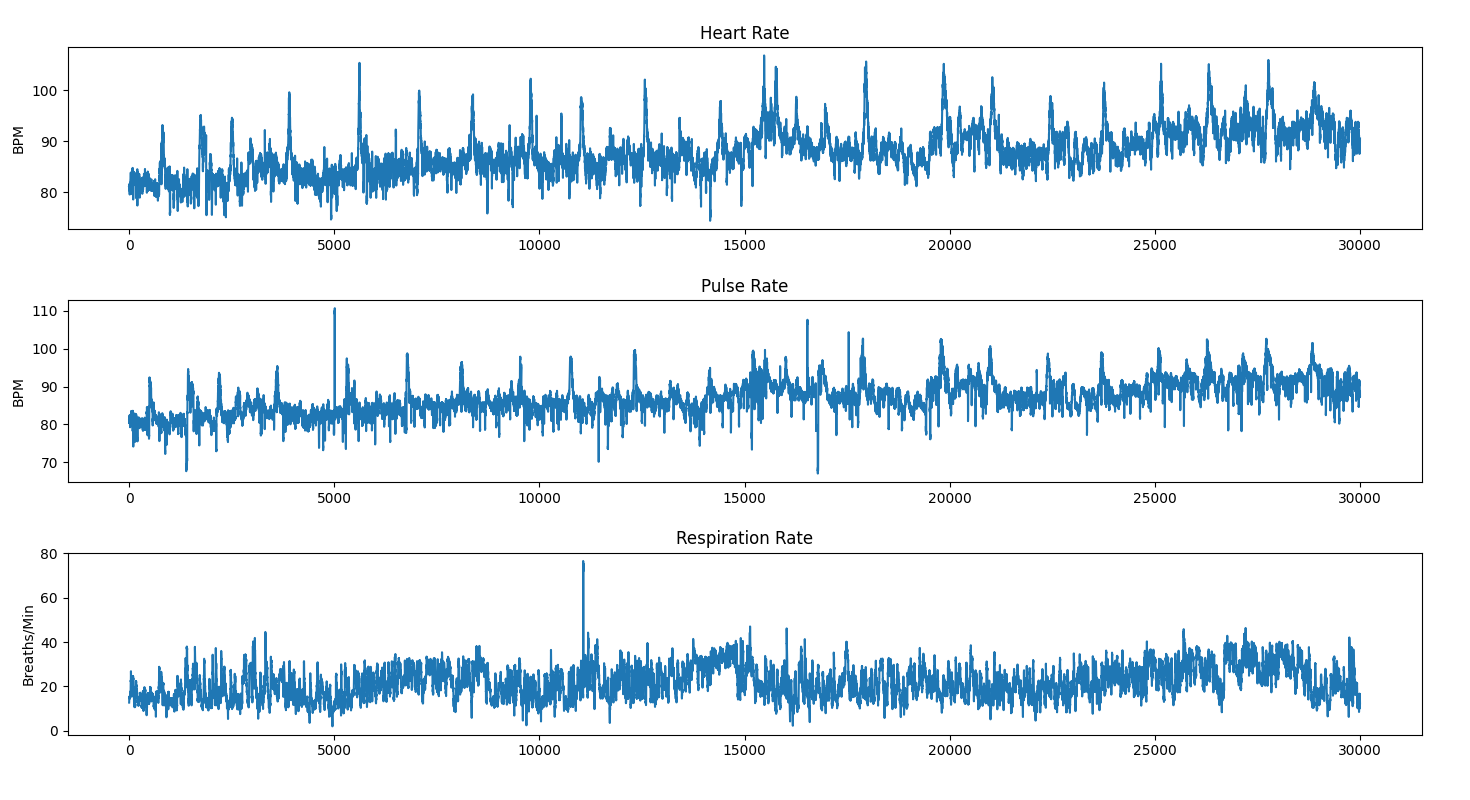
\includegraphics[scale=0.45]{plot.png}

\end{document}